% Template for PLoS
% Version 3.4 January 2017
\documentclass[10pt,letterpaper]{article}
\usepackage[top=0.85in,left=2.75in,footskip=0.75in]{geometry}

% amsmath and amssymb packages, useful for mathematical formulas and symbols
\usepackage{amsmath,amssymb}

% Use adjustwidth environment to exceed column width (see example table in text)
\usepackage{changepage}

% Use Unicode characters when possible
\usepackage[utf8x]{inputenc}

% textcomp package and marvosym package for additional characters
\usepackage{textcomp,marvosym}

% cite package, to clean up citations in the main text. Do not remove.
% \usepackage{cite}

% Use nameref to cite supporting information files (see Supporting Information section for more info)
\usepackage{nameref,hyperref}

% line numbers
\usepackage[right]{lineno}

% ligatures disabled
\usepackage{microtype}
\DisableLigatures[f]{encoding = *, family = * }

% color can be used to apply background shading to table cells only
\usepackage[table]{xcolor}

% array package and thick rules for tables
\usepackage{array}

% create "+" rule type for thick vertical lines
\newcolumntype{+}{!{\vrule width 2pt}}

% create \thickcline for thick horizontal lines of variable length
\newlength\savedwidth
\newcommand\thickcline[1]{%
  \noalign{\global\savedwidth\arrayrulewidth\global\arrayrulewidth 2pt}%
  \cline{#1}%
  \noalign{\vskip\arrayrulewidth}%
  \noalign{\global\arrayrulewidth\savedwidth}%
}

% \thickhline command for thick horizontal lines that span the table
\newcommand\thickhline{\noalign{\global\savedwidth\arrayrulewidth\global\arrayrulewidth 2pt}%
\hline
\noalign{\global\arrayrulewidth\savedwidth}}


% Remove comment for double spacing
%\usepackage{setspace} 
%\doublespacing

% Text layout
\raggedright
\setlength{\parindent}{0.5cm}
\textwidth 5.25in 
\textheight 8.75in

% Bold the 'Figure #' in the caption and separate it from the title/caption with a period
% Captions will be left justified
\usepackage[aboveskip=1pt,labelfont=bf,labelsep=period,justification=raggedright,singlelinecheck=off]{caption}
\renewcommand{\figurename}{Fig}

% Use the PLoS provided BiBTeX style
% \bibliographystyle{plos2015}

% Remove brackets from numbering in List of References
\makeatletter
\renewcommand{\@biblabel}[1]{\quad#1.}
\makeatother

% Leave date blank
\date{}

% Header and Footer with logo
\usepackage{lastpage,fancyhdr,graphicx}
\usepackage{epstopdf}
\pagestyle{myheadings}
\pagestyle{fancy}
\fancyhf{}
\setlength{\headheight}{27.023pt}
\lhead{
\includegraphics[width=2.0in]{PLOS-submission.eps}}
\rfoot{\thepage/\pageref{LastPage}}
\renewcommand{\footrule}{\hrule height 2pt \vspace{2mm}}
\fancyheadoffset[L]{2.25in}
\fancyfootoffset[L]{2.25in}
\lfoot{\sf PLOS}

%% Include all macros below
\newcommand{\lorem}{{\bf LOREM}}
\newcommand{\ipsum}{{\bf IPSUM}}

\usepackage{color}
\usepackage{fancyvrb}
\newcommand{\VerbBar}{|}
\newcommand{\VERB}{\Verb[commandchars=\\\{\}]}
\DefineVerbatimEnvironment{Highlighting}{Verbatim}{commandchars=\\\{\}}
% Add ',fontsize=\small' for more characters per line
\usepackage{framed}
\definecolor{shadecolor}{RGB}{248,248,248}
\newenvironment{Shaded}{\begin{snugshade}}{\end{snugshade}}
\newcommand{\KeywordTok}[1]{\textcolor[rgb]{0.13,0.29,0.53}{\textbf{#1}}}
\newcommand{\DataTypeTok}[1]{\textcolor[rgb]{0.13,0.29,0.53}{#1}}
\newcommand{\DecValTok}[1]{\textcolor[rgb]{0.00,0.00,0.81}{#1}}
\newcommand{\BaseNTok}[1]{\textcolor[rgb]{0.00,0.00,0.81}{#1}}
\newcommand{\FloatTok}[1]{\textcolor[rgb]{0.00,0.00,0.81}{#1}}
\newcommand{\ConstantTok}[1]{\textcolor[rgb]{0.00,0.00,0.00}{#1}}
\newcommand{\CharTok}[1]{\textcolor[rgb]{0.31,0.60,0.02}{#1}}
\newcommand{\SpecialCharTok}[1]{\textcolor[rgb]{0.00,0.00,0.00}{#1}}
\newcommand{\StringTok}[1]{\textcolor[rgb]{0.31,0.60,0.02}{#1}}
\newcommand{\VerbatimStringTok}[1]{\textcolor[rgb]{0.31,0.60,0.02}{#1}}
\newcommand{\SpecialStringTok}[1]{\textcolor[rgb]{0.31,0.60,0.02}{#1}}
\newcommand{\ImportTok}[1]{#1}
\newcommand{\CommentTok}[1]{\textcolor[rgb]{0.56,0.35,0.01}{\textit{#1}}}
\newcommand{\DocumentationTok}[1]{\textcolor[rgb]{0.56,0.35,0.01}{\textbf{\textit{#1}}}}
\newcommand{\AnnotationTok}[1]{\textcolor[rgb]{0.56,0.35,0.01}{\textbf{\textit{#1}}}}
\newcommand{\CommentVarTok}[1]{\textcolor[rgb]{0.56,0.35,0.01}{\textbf{\textit{#1}}}}
\newcommand{\OtherTok}[1]{\textcolor[rgb]{0.56,0.35,0.01}{#1}}
\newcommand{\FunctionTok}[1]{\textcolor[rgb]{0.00,0.00,0.00}{#1}}
\newcommand{\VariableTok}[1]{\textcolor[rgb]{0.00,0.00,0.00}{#1}}
\newcommand{\ControlFlowTok}[1]{\textcolor[rgb]{0.13,0.29,0.53}{\textbf{#1}}}
\newcommand{\OperatorTok}[1]{\textcolor[rgb]{0.81,0.36,0.00}{\textbf{#1}}}
\newcommand{\BuiltInTok}[1]{#1}
\newcommand{\ExtensionTok}[1]{#1}
\newcommand{\PreprocessorTok}[1]{\textcolor[rgb]{0.56,0.35,0.01}{\textit{#1}}}
\newcommand{\AttributeTok}[1]{\textcolor[rgb]{0.77,0.63,0.00}{#1}}
\newcommand{\RegionMarkerTok}[1]{#1}
\newcommand{\InformationTok}[1]{\textcolor[rgb]{0.56,0.35,0.01}{\textbf{\textit{#1}}}}
\newcommand{\WarningTok}[1]{\textcolor[rgb]{0.56,0.35,0.01}{\textbf{\textit{#1}}}}
\newcommand{\AlertTok}[1]{\textcolor[rgb]{0.94,0.16,0.16}{#1}}
\newcommand{\ErrorTok}[1]{\textcolor[rgb]{0.64,0.00,0.00}{\textbf{#1}}}
\newcommand{\NormalTok}[1]{#1}




\usepackage{forarray}
\usepackage{xstring}
\newcommand{\getIndex}[2]{
  \ForEach{,}{\IfEq{#1}{\thislevelitem}{\number\thislevelcount\ExitForEach}{}}{#2}
}

\setcounter{secnumdepth}{0}

\newcommand{\getAff}[1]{
  \getIndex{#1}{}
}

\providecommand{\tightlist}{%
  \setlength{\itemsep}{0pt}\setlength{\parskip}{0pt}}

\begin{document}
\vspace*{0.2in}

% Title must be 250 characters or less.
\begin{flushleft}
{\Large
\textbf\newline{NRSG 741 Homework 6} % Please use "sentence case" for title and headings (capitalize only the first word in a title (or heading), the first word in a subtitle (or subheading), and any proper nouns).
}
\newline
\\
Tommy Flynn\textsuperscript{\getAff{Emory University}}\\
\bigskip
\bigskip
\end{flushleft}
% Please keep the abstract below 300 words
\section*{Abstract}
Homework 6 was due on 04/06/2018, the same day as my F-31 NRSA
application. I wasn't able to complete both. My apologies for being late
on this assignment. I wanted to get it done anyway, so I don't get
behind. Thanks.

% Please keep the Author Summary between 150 and 200 words
% Use first person. PLOS ONE authors please skip this step. 
% Author Summary not valid for PLOS ONE submissions.   

\linenumbers

% Use "Eq" instead of "Equation" for equation citations.
\emph{Find the associated GitHub Repository Here:
\url{https://github.com/tommyflynn/N741_Homework/tree/master/Flynn_HW_06}}

For homework 6, we use the \textbf{HELP} (Health Evaluation and Linkage
to Primary Care) Dataset.

\subsubsection{Variables for Homework 6}\label{variables-for-homework-6}

Only on the following variables from the HELP dataset are used for this
assignment:

\begin{longtable}[]{@{}ll@{}}
\caption{Use these variables from HELP dataset for Homework
06}\tabularnewline
\toprule
& Variable Label\tabularnewline
\midrule
\endfirsthead
\toprule
& Variable Label\tabularnewline
\midrule
\endhead
age & Age at baseline (in years)\tabularnewline
female & Gender of respondent\tabularnewline
pss\_fr & Perceived Social Support - friends\tabularnewline
homeless & One or more nights on the street or shelter in past 6
months\tabularnewline
pcs & SF36 Physical Composite Score - Baseline\tabularnewline
mcs & SF36 Mental Composite Score - Baseline\tabularnewline
cesd & CESD total score - Baseline\tabularnewline
\bottomrule
\end{longtable}

\subsection{Homework 6 Assignment}\label{homework-6-assignment}

For Homework 6, you will be looking at depression in these subjects.
First, you will be running a model to look at the continuous depression
measure - the CESD \href{http://cesd-r.com/}{Center for Epidemiologic
Studies Depression Scale} which is a measure of depressive symptoms.
Also see the APA details on the CESD at
\url{http://www.apa.org/pi/about/publications/caregivers/practice-settings/assessment/tools/depression-scale.aspx}.
The CESD can be used to predict actual clinical depression but it is not
technically a diagnosis of depression. The CESD scores range from 0 (no
depressive symptoms) to 60 (most severe depressive symptoms). You will
use the (\texttt{cesd}) variable to run a linear regression.

The recommended threshold used to indicate potential clinical depression
is for people with scores of 16 or greater. You will then use the
variable created using this cutoff (\texttt{cesd\_gte16}) to perform a
similar modeling approach with the variables to predict the probability
of clinical depression (using logistic regression).

\subsubsection{\texorpdfstring{1. {[}Model 1{]} Run a simple linear
regression (\texttt{lm()}) for \texttt{cesd} using the \texttt{mcs}
variable, which is the mental component quality of life score from the
SF36.}{1. {[}Model 1{]} Run a simple linear regression (lm()) for cesd using the mcs variable, which is the mental component quality of life score from the SF36.}}\label{model-1-run-a-simple-linear-regression-lm-for-cesd-using-the-mcs-variable-which-is-the-mental-component-quality-of-life-score-from-the-sf36.}

\begin{Shaded}
\begin{Highlighting}[]
\NormalTok{reg1 <-}\StringTok{ }\KeywordTok{lm}\NormalTok{(cesd }\OperatorTok{~}\StringTok{ }\NormalTok{mcs, }\DataTypeTok{data =}\NormalTok{ h1)}
\KeywordTok{summary}\NormalTok{(reg1)}
\end{Highlighting}
\end{Shaded}

\begin{verbatim}
## 
## Call:
## lm(formula = cesd ~ mcs, data = h1)
## 
## Residuals:
##      Min       1Q   Median       3Q      Max 
## -27.3593  -6.7277  -0.0024   6.2374  24.4239 
## 
## Coefficients:
##             Estimate Std. Error t value Pr(>|t|)    
## (Intercept) 53.90219    1.14723   46.98   <2e-16 ***
## mcs         -0.66467    0.03357  -19.80   <2e-16 ***
## ---
## Signif. codes:  0 '***' 0.001 '**' 0.01 '*' 0.05 '.' 0.1 ' ' 1
## 
## Residual standard error: 9.164 on 451 degrees of freedom
## Multiple R-squared:  0.465,  Adjusted R-squared:  0.4638 
## F-statistic:   392 on 1 and 451 DF,  p-value: < 2.2e-16
\end{verbatim}

\begin{Shaded}
\begin{Highlighting}[]
\KeywordTok{plot}\NormalTok{(cesd }\OperatorTok{~}\StringTok{ }\NormalTok{mcs, }\DataTypeTok{data=}\NormalTok{h1)}
\KeywordTok{abline}\NormalTok{(}\DataTypeTok{a=}\FloatTok{53.902}\NormalTok{, }\DataTypeTok{b=}\OperatorTok{-}\FloatTok{0.665}\NormalTok{)}
\end{Highlighting}
\end{Shaded}

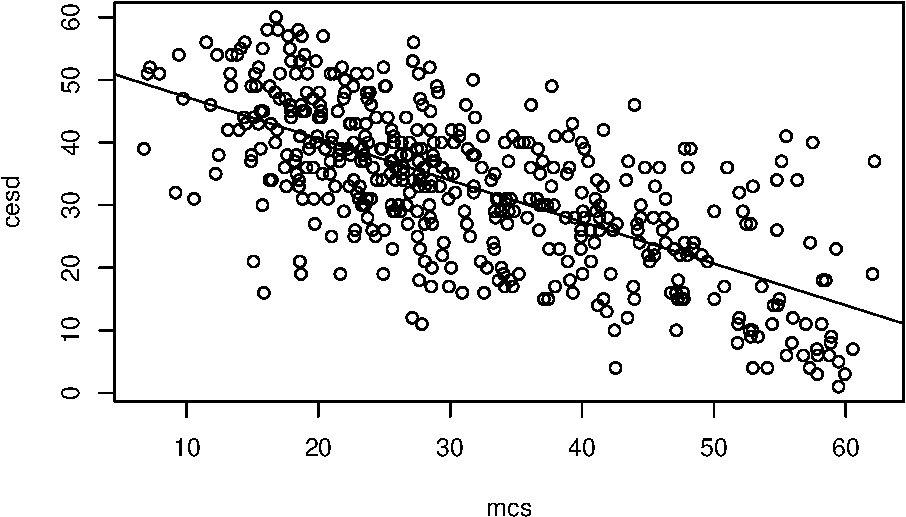
\includegraphics{Flynn_HW_06_files/figure-latex/answer 1-1.pdf}

\subsubsection{2. Write the equation of the final fitted model
(i.e.~what is the intercept and the slope)? Write a sentence describing
the model results (interpret the intercept and
slope).}\label{write-the-equation-of-the-final-fitted-model-i.e.what-is-the-intercept-and-the-slope-write-a-sentence-describing-the-model-results-interpret-the-intercept-and-slope.}

\begin{equation}
  cesd = 53.902 - (0.665)mcs
\end{equation}

\textbf{For each unit increase in \texttt{mcs}, the \texttt{cesd} score
decreases by 0.665 units.}

\subsubsection{\texorpdfstring{3. How much variability in the
\texttt{cesd} does the \texttt{mcs} explain? (what is the R2?) Write a
sentence describing how well the \texttt{mcs} does in predicting the
\texttt{cesd}.}{3. How much variability in the cesd does the mcs explain? (what is the R2?) Write a sentence describing how well the mcs does in predicting the cesd.}}\label{how-much-variability-in-the-cesd-does-the-mcs-explain-what-is-the-r2-write-a-sentence-describing-how-well-the-mcs-does-in-predicting-the-cesd.}

\textbf{46\% of the variability in \texttt{cesd} is due to \texttt{mcs}
(R2=0.47).}

\subsubsection{\texorpdfstring{4. {[}Model 2{]} Run a second linear
regression model (\texttt{lm()}) for the \texttt{cesd} putting in all of
the other
variables:}{4. {[}Model 2{]} Run a second linear regression model (lm()) for the cesd putting in all of the other variables:}}\label{model-2-run-a-second-linear-regression-model-lm-for-the-cesd-putting-in-all-of-the-other-variables}

\begin{Shaded}
\begin{Highlighting}[]
\NormalTok{model1 <-}\StringTok{ }\KeywordTok{lm}\NormalTok{(cesd }\OperatorTok{~}\StringTok{ }\NormalTok{age }\OperatorTok{+}\StringTok{ }\NormalTok{female }\OperatorTok{+}\StringTok{ }\NormalTok{pss_fr }\OperatorTok{+}\StringTok{ }\NormalTok{homeless }\OperatorTok{+}\StringTok{ }\NormalTok{pcs }\OperatorTok{+}\StringTok{ }\NormalTok{mcs, }\DataTypeTok{data=}\NormalTok{h1)}
    
\CommentTok{#Print out the model results with the coefficients and tests and model fit statistics.}
\KeywordTok{summary}\NormalTok{(model1)}
\end{Highlighting}
\end{Shaded}

\begin{verbatim}
## 
## Call:
## lm(formula = cesd ~ age + female + pss_fr + homeless + pcs + 
##     mcs, data = h1)
## 
## Residuals:
##      Min       1Q   Median       3Q      Max 
## -25.1711  -5.9894  -0.2077   5.5706  27.3137 
## 
## Coefficients:
##             Estimate Std. Error t value Pr(>|t|)    
## (Intercept) 65.30046    3.18670  20.492  < 2e-16 ***
## age         -0.01348    0.05501  -0.245   0.8065    
## female       2.35028    0.98810   2.379   0.0178 *  
## pss_fr      -0.25569    0.10567  -2.420   0.0159 *  
## homeless     0.46545    0.84261   0.552   0.5810    
## pcs         -0.23639    0.03987  -5.929  6.1e-09 ***
## mcs         -0.62093    0.03261 -19.042  < 2e-16 ***
## ---
## Signif. codes:  0 '***' 0.001 '**' 0.01 '*' 0.05 '.' 0.1 ' ' 1
## 
## Residual standard error: 8.683 on 446 degrees of freedom
## Multiple R-squared:  0.5249, Adjusted R-squared:  0.5185 
## F-statistic: 82.14 on 6 and 446 DF,  p-value: < 2.2e-16
\end{verbatim}

\subsubsection{5. Which variables are significant in the model? Write a
sentence or two describing the impact of these variables for predicting
depression scores (HINT: interpret the coefficient
terms).}\label{which-variables-are-significant-in-the-model-write-a-sentence-or-two-describing-the-impact-of-these-variables-for-predicting-depression-scores-hint-interpret-the-coefficient-terms.}

\textbf{\texttt{Female,\ pss\_fr,\ pcs} and \texttt{mcs} are all
significantly associated with \texttt{cesd}. On average, women score
higher on the \texttt{cesd} by 2.34 points, every unit increase on the
physical composite score decreases the \texttt{cesd} score by 0.24, a
unit increase on the mental composite score decreases \texttt{cesd} by
0.62 unites, and 1 unit increase on the social support scale decreased
\texttt{cesd} by 0.26 units.}

\subsubsection{\texorpdfstring{6. Following the example we did in class
for the Prestige dataset
\url{https://cdn.rawgit.com/vhertzb/2018week9/2f2ea142/2018week9.html?raw=true},
generate the diagnostic plotss for this model with these 6 predictors
(e.g.~get the residual plot by variables, the added-variable plots, the
Q-Q plot, diagnostic plots). Also run the VIFs to check for
multicollinearity
issues.}{6. Following the example we did in class for the Prestige dataset https://cdn.rawgit.com/vhertzb/2018week9/2f2ea142/2018week9.html?raw=true, generate the diagnostic plotss for this model with these 6 predictors (e.g.~get the residual plot by variables, the added-variable plots, the Q-Q plot, diagnostic plots). Also run the VIFs to check for multicollinearity issues.}}\label{following-the-example-we-did-in-class-for-the-prestige-dataset-httpscdn.rawgit.comvhertzb2018week92f2ea1422018week9.htmlrawtrue-generate-the-diagnostic-plotss-for-this-model-with-these-6-predictors-e.g.get-the-residual-plot-by-variables-the-added-variable-plots-the-q-q-plot-diagnostic-plots.-also-run-the-vifs-to-check-for-multicollinearity-issues.}

\subsubsection{\texorpdfstring{7. {[}Model 3{]} Repeat Model 1 above,
except this time run a logistic regression (\texttt{glm()}) to predict
CESD scores =\textgreater{} 16 (using the \texttt{cesd\_gte16} as the
outcome) as a function of \texttt{mcs} scores. Show a summary of the
final fitted model and explain the coefficients. {[}\textbf{REMEMBER} to
compute the Odds Ratios after you get the raw coefficient
(betas){]}.}{7. {[}Model 3{]} Repeat Model 1 above, except this time run a logistic regression (glm()) to predict CESD scores =\textgreater{} 16 (using the cesd\_gte16 as the outcome) as a function of mcs scores. Show a summary of the final fitted model and explain the coefficients. {[}REMEMBER to compute the Odds Ratios after you get the raw coefficient (betas){]}.}}\label{model-3-repeat-model-1-above-except-this-time-run-a-logistic-regression-glm-to-predict-cesd-scores-16-using-the-cesd_gte16-as-the-outcome-as-a-function-of-mcs-scores.-show-a-summary-of-the-final-fitted-model-and-explain-the-coefficients.-remember-to-compute-the-odds-ratios-after-you-get-the-raw-coefficient-betas.}

\subsubsection{\texorpdfstring{8. Use the \texttt{predict()} function
like we did in class to predict CESD =\textgreater{} 16 and compare it
back to the original data. For now, use a cutoff probability of 0.5 - if
the probability is \textgreater{} 0.5 consider this to be true and false
otherwise. Like we did in class. \textbf{REMEMBER} See the R code for
the class example at
\url{https://github.com/melindahiggins2000/N741_lecture11_27March2018/blob/master/lesson11_logreg_Rcode.R}}{8. Use the predict() function like we did in class to predict CESD =\textgreater{} 16 and compare it back to the original data. For now, use a cutoff probability of 0.5 - if the probability is \textgreater{} 0.5 consider this to be true and false otherwise. Like we did in class. REMEMBER See the R code for the class example at https://github.com/melindahiggins2000/N741\_lecture11\_27March2018/blob/master/lesson11\_logreg\_Rcode.R}}\label{use-the-predict-function-like-we-did-in-class-to-predict-cesd-16-and-compare-it-back-to-the-original-data.-for-now-use-a-cutoff-probability-of-0.5---if-the-probability-is-0.5-consider-this-to-be-true-and-false-otherwise.-like-we-did-in-class.-remember-see-the-r-code-for-the-class-example-at-httpsgithub.commelindahiggins2000n741_lecture11_27march2018blobmasterlesson11_logreg_rcode.r}

\begin{verbatim}
+ How well did the model correctly predict CESD scores => 16 (indicating depression)? (make the "confusion matrix" and look at the true positives and true negatives versus the false positives and false negatives).
\end{verbatim}

\subsubsection{9. Make an ROC curve plot and compute the AUC and explain
if this is a good model for predicting depression or
not}\label{make-an-roc-curve-plot-and-compute-the-auc-and-explain-if-this-is-a-good-model-for-predicting-depression-or-not}

\subsubsection{\texorpdfstring{10. Make a plot showing the probability
curve - put the \texttt{mcs} values on the X-axis and the probability of
depression on the Y-axis. Based on this plot, do you think the
\texttt{mcs} is a good predictor of depression? {[}\textbf{FYI} This
plot is also called an ``effect plot'' is you're using \texttt{Rcmdr} to
do these
analyses.{]}}{10. Make a plot showing the probability curve - put the mcs values on the X-axis and the probability of depression on the Y-axis. Based on this plot, do you think the mcs is a good predictor of depression? {[}FYI This plot is also called an effect plot is you're using Rcmdr to do these analyses.{]}}}\label{make-a-plot-showing-the-probability-curve---put-the-mcs-values-on-the-x-axis-and-the-probability-of-depression-on-the-y-axis.-based-on-this-plot-do-you-think-the-mcs-is-a-good-predictor-of-depression-fyi-this-plot-is-also-called-an-effect-plot-is-youre-using-rcmdr-to-do-these-analyses.}

\begin{center}\rule{0.5\linewidth}{\linethickness}\end{center}

\nolinenumbers


\end{document}

